


\tikzset{every picture/.style={line width=0.75pt}} %set default line width to 0.75pt        

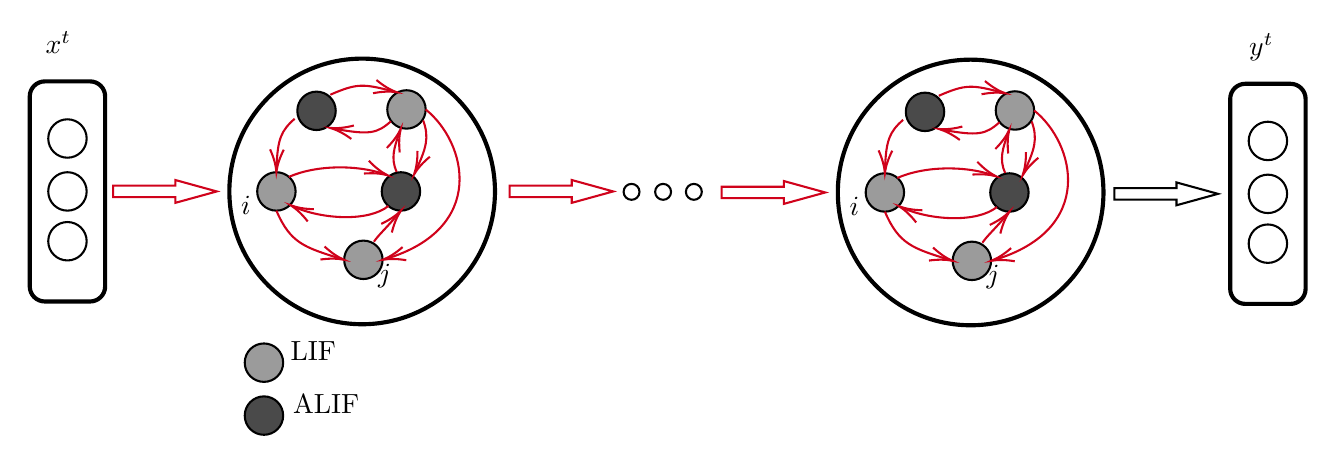
\begin{tikzpicture}[x=0.75pt,y=0.75pt,yscale=-1,xscale=1]
%uncomment if require: \path (0,287); %set diagram left start at 0, and has height of 287

%Rounded Rect [id:dp5125213371166828] 
\draw  [line width=1.5]  (2,112.71) .. controls (2,108.7) and (5.25,105.45) .. (9.27,105.45) -- (31.07,105.45) .. controls (35.08,105.45) and (38.33,108.7) .. (38.33,112.71) -- (38.33,204.22) .. controls (38.33,208.23) and (35.08,211.49) .. (31.07,211.49) -- (9.27,211.49) .. controls (5.25,211.49) and (2,208.23) .. (2,204.22) -- cycle ;
%Shape: Circle [id:dp1036864356471725] 
\draw   (10.91,182.47) .. controls (10.91,177.36) and (15.06,173.21) .. (20.17,173.21) .. controls (25.28,173.21) and (29.42,177.36) .. (29.42,182.47) .. controls (29.42,187.58) and (25.28,191.72) .. (20.17,191.72) .. controls (15.06,191.72) and (10.91,187.58) .. (10.91,182.47) -- cycle ;
%Shape: Circle [id:dp6658728805120719] 
\draw   (10.91,132.97) .. controls (10.91,127.86) and (15.06,123.71) .. (20.17,123.71) .. controls (25.28,123.71) and (29.42,127.86) .. (29.42,132.97) .. controls (29.42,138.08) and (25.28,142.22) .. (20.17,142.22) .. controls (15.06,142.22) and (10.91,138.08) .. (10.91,132.97) -- cycle ;
%Right Arrow [id:dp741109303104662] 
\draw  [color={rgb, 255:red, 208; green, 2; blue, 27 }  ,draw opacity=1 ] (42.17,155.71) -- (72.13,155.71) -- (72.13,152.96) -- (92.11,158.47) -- (72.13,163.97) -- (72.13,161.22) -- (42.17,161.22) -- cycle ;
%Shape: Circle [id:dp6585629105990938] 
\draw  [color={rgb, 255:red, 0; green, 0; blue, 0 }  ,draw opacity=1 ][line width=1.5]  (98.17,158.47) .. controls (98.17,123.13) and (126.82,94.48) .. (162.15,94.48) .. controls (197.49,94.48) and (226.14,123.13) .. (226.14,158.47) .. controls (226.14,193.81) and (197.49,222.45) .. (162.15,222.45) .. controls (126.82,222.45) and (98.17,193.81) .. (98.17,158.47) -- cycle ;
%Shape: Circle [id:dp741227979850853] 
\draw  [fill={rgb, 255:red, 74; green, 74; blue, 74 }  ,fill opacity=1 ] (130.91,119.63) .. controls (130.91,114.52) and (135.06,110.38) .. (140.17,110.38) .. controls (145.28,110.38) and (149.42,114.52) .. (149.42,119.63) .. controls (149.42,124.74) and (145.28,128.89) .. (140.17,128.89) .. controls (135.06,128.89) and (130.91,124.74) .. (130.91,119.63) -- cycle ;
%Shape: Circle [id:dp7307755920673902] 
\draw  [fill={rgb, 255:red, 155; green, 155; blue, 155 }  ,fill opacity=1 ] (174.25,118.97) .. controls (174.25,113.86) and (178.39,109.71) .. (183.5,109.71) .. controls (188.61,109.71) and (192.75,113.86) .. (192.75,118.97) .. controls (192.75,124.08) and (188.61,128.22) .. (183.5,128.22) .. controls (178.39,128.22) and (174.25,124.08) .. (174.25,118.97) -- cycle ;
%Shape: Circle [id:dp39480228938683437] 
\draw  [fill={rgb, 255:red, 155; green, 155; blue, 155 }  ,fill opacity=1 ] (111.58,158.47) .. controls (111.58,153.36) and (115.72,149.21) .. (120.83,149.21) .. controls (125.94,149.21) and (130.09,153.36) .. (130.09,158.47) .. controls (130.09,163.58) and (125.94,167.72) .. (120.83,167.72) .. controls (115.72,167.72) and (111.58,163.58) .. (111.58,158.47) -- cycle ;
%Shape: Circle [id:dp707851840639744] 
\draw  [fill={rgb, 255:red, 74; green, 74; blue, 74 }  ,fill opacity=1 ] (171.58,158.47) .. controls (171.58,153.36) and (175.72,149.21) .. (180.83,149.21) .. controls (185.94,149.21) and (190.09,153.36) .. (190.09,158.47) .. controls (190.09,163.58) and (185.94,167.72) .. (180.83,167.72) .. controls (175.72,167.72) and (171.58,163.58) .. (171.58,158.47) -- cycle ;
%Shape: Circle [id:dp5633766668791496] 
\draw  [fill={rgb, 255:red, 155; green, 155; blue, 155 }  ,fill opacity=1 ] (153.49,191.41) .. controls (153.49,186.3) and (157.64,182.16) .. (162.75,182.16) .. controls (167.86,182.16) and (172,186.3) .. (172,191.41) .. controls (172,196.52) and (167.86,200.67) .. (162.75,200.67) .. controls (157.64,200.67) and (153.49,196.52) .. (153.49,191.41) -- cycle ;
%Curve Lines [id:da5654601008343274] 
\draw [color={rgb, 255:red, 208; green, 2; blue, 27 }  ,draw opacity=1 ]   (120.83,167.72) .. controls (127.61,183.41) and (134.21,185.38) .. (151.83,190.89) ;
\draw [shift={(153.49,191.41)}, rotate = 197.41] [color={rgb, 255:red, 208; green, 2; blue, 27 }  ,draw opacity=1 ][line width=0.75]    (10.93,-3.29) .. controls (6.95,-1.4) and (3.31,-0.3) .. (0,0) .. controls (3.31,0.3) and (6.95,1.4) .. (10.93,3.29)   ;
%Curve Lines [id:da8424508537757602] 
\draw [color={rgb, 255:red, 208; green, 2; blue, 27 }  ,draw opacity=1 ]   (126.81,151.48) .. controls (139.8,145.75) and (158.99,145.49) .. (172.54,150.01) ;
\draw [shift={(174.41,150.68)}, rotate = 200.92000000000002] [color={rgb, 255:red, 208; green, 2; blue, 27 }  ,draw opacity=1 ][line width=0.75]    (10.93,-3.29) .. controls (6.95,-1.4) and (3.31,-0.3) .. (0,0) .. controls (3.31,0.3) and (6.95,1.4) .. (10.93,3.29)   ;
%Curve Lines [id:da8098070733054574] 
\draw [color={rgb, 255:red, 208; green, 2; blue, 27 }  ,draw opacity=1 ]   (174.81,165.48) .. controls (165.21,173.16) and (143.08,171.99) .. (129.29,165.87) ;
\draw [shift={(127.61,165.08)}, rotate = 386.57] [color={rgb, 255:red, 208; green, 2; blue, 27 }  ,draw opacity=1 ][line width=0.75]    (10.93,-3.29) .. controls (6.95,-1.4) and (3.31,-0.3) .. (0,0) .. controls (3.31,0.3) and (6.95,1.4) .. (10.93,3.29)   ;
%Curve Lines [id:da5891979583346552] 
\draw [color={rgb, 255:red, 208; green, 2; blue, 27 }  ,draw opacity=1 ]   (146.81,111.88) .. controls (159.87,106.12) and (162.97,106.62) .. (177,110.21) ;
\draw [shift={(178.81,110.68)}, rotate = 194.38] [color={rgb, 255:red, 208; green, 2; blue, 27 }  ,draw opacity=1 ][line width=0.75]    (10.93,-3.29) .. controls (6.95,-1.4) and (3.31,-0.3) .. (0,0) .. controls (3.31,0.3) and (6.95,1.4) .. (10.93,3.29)   ;
%Curve Lines [id:da264987914027079] 
\draw [color={rgb, 255:red, 208; green, 2; blue, 27 }  ,draw opacity=1 ]   (178.76,149.08) .. controls (175.82,142.45) and (177.61,137.18) .. (180.1,130.15) ;
\draw [shift={(180.76,128.28)}, rotate = 469.29] [color={rgb, 255:red, 208; green, 2; blue, 27 }  ,draw opacity=1 ][line width=0.75]    (10.93,-3.29) .. controls (6.95,-1.4) and (3.31,-0.3) .. (0,0) .. controls (3.31,0.3) and (6.95,1.4) .. (10.93,3.29)   ;
%Curve Lines [id:da17823983207616156] 
\draw [color={rgb, 255:red, 208; green, 2; blue, 27 }  ,draw opacity=1 ]   (129.61,123.48) .. controls (123.08,129.24) and (121.35,133.15) .. (120.89,147.38) ;
\draw [shift={(120.83,149.21)}, rotate = 271.38] [color={rgb, 255:red, 208; green, 2; blue, 27 }  ,draw opacity=1 ][line width=0.75]    (10.93,-3.29) .. controls (6.95,-1.4) and (3.31,-0.3) .. (0,0) .. controls (3.31,0.3) and (6.95,1.4) .. (10.93,3.29)   ;
%Curve Lines [id:da7421559076195556] 
\draw [color={rgb, 255:red, 208; green, 2; blue, 27 }  ,draw opacity=1 ]   (167.81,182.69) .. controls (170.45,178.93) and (173.43,176.59) .. (179.61,169.2) ;
\draw [shift={(180.83,167.72)}, rotate = 489.31] [color={rgb, 255:red, 208; green, 2; blue, 27 }  ,draw opacity=1 ][line width=0.75]    (10.93,-3.29) .. controls (6.95,-1.4) and (3.31,-0.3) .. (0,0) .. controls (3.31,0.3) and (6.95,1.4) .. (10.93,3.29)   ;
%Curve Lines [id:da4256075721549528] 
\draw [color={rgb, 255:red, 208; green, 2; blue, 27 }  ,draw opacity=1 ]   (176.01,124.68) .. controls (169.45,130.47) and (165.87,131.42) .. (148.73,128.24) ;
\draw [shift={(146.81,127.88)}, rotate = 370.84000000000003] [color={rgb, 255:red, 208; green, 2; blue, 27 }  ,draw opacity=1 ][line width=0.75]    (10.93,-3.29) .. controls (6.95,-1.4) and (3.31,-0.3) .. (0,0) .. controls (3.31,0.3) and (6.95,1.4) .. (10.93,3.29)   ;
%Shape: Circle [id:dp8922241675489593] 
\draw  [fill={rgb, 255:red, 74; green, 74; blue, 74 }  ,fill opacity=1 ] (105.58,266.47) .. controls (105.58,261.36) and (109.72,257.21) .. (114.83,257.21) .. controls (119.94,257.21) and (124.09,261.36) .. (124.09,266.47) .. controls (124.09,271.58) and (119.94,275.72) .. (114.83,275.72) .. controls (109.72,275.72) and (105.58,271.58) .. (105.58,266.47) -- cycle ;
%Shape: Circle [id:dp07237313980777427] 
\draw  [fill={rgb, 255:red, 155; green, 155; blue, 155 }  ,fill opacity=1 ] (105.58,240.97) .. controls (105.58,235.86) and (109.72,231.71) .. (114.83,231.71) .. controls (119.94,231.71) and (124.09,235.86) .. (124.09,240.97) .. controls (124.09,246.08) and (119.94,250.22) .. (114.83,250.22) .. controls (109.72,250.22) and (105.58,246.08) .. (105.58,240.97) -- cycle ;
%Right Arrow [id:dp7348532029334156] 
\draw  [color={rgb, 255:red, 0; green, 0; blue, 0 }  ,draw opacity=1 ] (524.53,156.88) -- (554.5,156.88) -- (554.5,154.13) -- (574.48,159.63) -- (554.5,165.14) -- (554.5,162.39) -- (524.53,162.39) -- cycle ;
%Shape: Circle [id:dp026235667443113897] 
\draw   (10.91,158.47) .. controls (10.91,153.36) and (15.06,149.21) .. (20.17,149.21) .. controls (25.28,149.21) and (29.42,153.36) .. (29.42,158.47) .. controls (29.42,163.58) and (25.28,167.72) .. (20.17,167.72) .. controls (15.06,167.72) and (10.91,163.58) .. (10.91,158.47) -- cycle ;
%Rounded Rect [id:dp8136688725026966] 
\draw  [line width=1.5]  (580.37,113.88) .. controls (580.37,109.87) and (583.62,106.61) .. (587.63,106.61) -- (609.43,106.61) .. controls (613.45,106.61) and (616.7,109.87) .. (616.7,113.88) -- (616.7,205.39) .. controls (616.7,209.4) and (613.45,212.65) .. (609.43,212.65) -- (587.63,212.65) .. controls (583.62,212.65) and (580.37,209.4) .. (580.37,205.39) -- cycle ;
%Shape: Circle [id:dp11133772958248556] 
\draw   (589.28,183.63) .. controls (589.28,178.52) and (593.42,174.38) .. (598.53,174.38) .. controls (603.64,174.38) and (607.79,178.52) .. (607.79,183.63) .. controls (607.79,188.74) and (603.64,192.89) .. (598.53,192.89) .. controls (593.42,192.89) and (589.28,188.74) .. (589.28,183.63) -- cycle ;
%Shape: Circle [id:dp9075431994144578] 
\draw   (589.28,134.13) .. controls (589.28,129.02) and (593.42,124.88) .. (598.53,124.88) .. controls (603.64,124.88) and (607.79,129.02) .. (607.79,134.13) .. controls (607.79,139.24) and (603.64,143.39) .. (598.53,143.39) .. controls (593.42,143.39) and (589.28,139.24) .. (589.28,134.13) -- cycle ;
%Shape: Circle [id:dp30918690373576596] 
\draw   (589.28,159.63) .. controls (589.28,154.52) and (593.42,150.38) .. (598.53,150.38) .. controls (603.64,150.38) and (607.79,154.52) .. (607.79,159.63) .. controls (607.79,164.74) and (603.64,168.89) .. (598.53,168.89) .. controls (593.42,168.89) and (589.28,164.74) .. (589.28,159.63) -- cycle ;
%Curve Lines [id:da005449794705521871] 
\draw [color={rgb, 255:red, 208; green, 2; blue, 27 }  ,draw opacity=1 ]   (192.75,118.97) .. controls (212.55,134.81) and (222.61,176.28) .. (173.51,190.98) ;
\draw [shift={(172,191.41)}, rotate = 344.28999999999996] [color={rgb, 255:red, 208; green, 2; blue, 27 }  ,draw opacity=1 ][line width=0.75]    (10.93,-3.29) .. controls (6.95,-1.4) and (3.31,-0.3) .. (0,0) .. controls (3.31,0.3) and (6.95,1.4) .. (10.93,3.29)   ;
%Curve Lines [id:da9608524955121955] 
\draw [color={rgb, 255:red, 208; green, 2; blue, 27 }  ,draw opacity=1 ]   (191.56,124.28) .. controls (194.6,132.64) and (192.95,137.75) .. (187.97,148.53) ;
\draw [shift={(187.16,150.28)}, rotate = 295.02] [color={rgb, 255:red, 208; green, 2; blue, 27 }  ,draw opacity=1 ][line width=0.75]    (10.93,-3.29) .. controls (6.95,-1.4) and (3.31,-0.3) .. (0,0) .. controls (3.31,0.3) and (6.95,1.4) .. (10.93,3.29)   ;
%Right Arrow [id:dp18193153290231412] 
\draw  [color={rgb, 255:red, 208; green, 2; blue, 27 }  ,draw opacity=1 ] (233.17,155.71) -- (263.13,155.71) -- (263.13,152.96) -- (283.11,158.47) -- (263.13,163.97) -- (263.13,161.22) -- (233.17,161.22) -- cycle ;
%Right Arrow [id:dp12547934202498445] 
\draw  [color={rgb, 255:red, 208; green, 2; blue, 27 }  ,draw opacity=1 ] (335.33,156.21) -- (365.3,156.21) -- (365.3,153.46) -- (385.28,158.97) -- (365.3,164.47) -- (365.3,161.72) -- (335.33,161.72) -- cycle ;
%Shape: Circle [id:dp2670612477818626] 
\draw  [color={rgb, 255:red, 0; green, 0; blue, 0 }  ,draw opacity=1 ][line width=1.5]  (391.33,158.97) .. controls (391.33,123.63) and (419.98,94.98) .. (455.32,94.98) .. controls (490.66,94.98) and (519.31,123.63) .. (519.31,158.97) .. controls (519.31,194.31) and (490.66,222.95) .. (455.32,222.95) .. controls (419.98,222.95) and (391.33,194.31) .. (391.33,158.97) -- cycle ;
%Shape: Circle [id:dp16625110004331534] 
\draw  [fill={rgb, 255:red, 74; green, 74; blue, 74 }  ,fill opacity=1 ] (424.08,120.13) .. controls (424.08,115.02) and (428.22,110.88) .. (433.33,110.88) .. controls (438.44,110.88) and (442.59,115.02) .. (442.59,120.13) .. controls (442.59,125.24) and (438.44,129.39) .. (433.33,129.39) .. controls (428.22,129.39) and (424.08,125.24) .. (424.08,120.13) -- cycle ;
%Shape: Circle [id:dp8348914065464377] 
\draw  [fill={rgb, 255:red, 155; green, 155; blue, 155 }  ,fill opacity=1 ] (467.41,119.47) .. controls (467.41,114.36) and (471.56,110.21) .. (476.67,110.21) .. controls (481.78,110.21) and (485.92,114.36) .. (485.92,119.47) .. controls (485.92,124.58) and (481.78,128.72) .. (476.67,128.72) .. controls (471.56,128.72) and (467.41,124.58) .. (467.41,119.47) -- cycle ;
%Shape: Circle [id:dp3479500590604021] 
\draw  [fill={rgb, 255:red, 155; green, 155; blue, 155 }  ,fill opacity=1 ] (404.75,158.97) .. controls (404.75,153.86) and (408.89,149.71) .. (414,149.71) .. controls (419.11,149.71) and (423.25,153.86) .. (423.25,158.97) .. controls (423.25,164.08) and (419.11,168.22) .. (414,168.22) .. controls (408.89,168.22) and (404.75,164.08) .. (404.75,158.97) -- cycle ;
%Shape: Circle [id:dp4006067412672085] 
\draw  [fill={rgb, 255:red, 74; green, 74; blue, 74 }  ,fill opacity=1 ] (464.75,158.97) .. controls (464.75,153.86) and (468.89,149.71) .. (474,149.71) .. controls (479.11,149.71) and (483.25,153.86) .. (483.25,158.97) .. controls (483.25,164.08) and (479.11,168.22) .. (474,168.22) .. controls (468.89,168.22) and (464.75,164.08) .. (464.75,158.97) -- cycle ;
%Shape: Circle [id:dp7049273904038411] 
\draw  [fill={rgb, 255:red, 155; green, 155; blue, 155 }  ,fill opacity=1 ] (446.66,191.91) .. controls (446.66,186.8) and (450.8,182.66) .. (455.91,182.66) .. controls (461.02,182.66) and (465.17,186.8) .. (465.17,191.91) .. controls (465.17,197.02) and (461.02,201.17) .. (455.91,201.17) .. controls (450.8,201.17) and (446.66,197.02) .. (446.66,191.91) -- cycle ;
%Curve Lines [id:da2730645645057217] 
\draw [color={rgb, 255:red, 208; green, 2; blue, 27 }  ,draw opacity=1 ]   (414,168.22) .. controls (420.77,183.91) and (427.37,185.88) .. (444.99,191.39) ;
\draw [shift={(446.66,191.91)}, rotate = 197.41] [color={rgb, 255:red, 208; green, 2; blue, 27 }  ,draw opacity=1 ][line width=0.75]    (10.93,-3.29) .. controls (6.95,-1.4) and (3.31,-0.3) .. (0,0) .. controls (3.31,0.3) and (6.95,1.4) .. (10.93,3.29)   ;
%Curve Lines [id:da0544716102889502] 
\draw [color={rgb, 255:red, 208; green, 2; blue, 27 }  ,draw opacity=1 ]   (419.98,151.98) .. controls (432.97,146.25) and (452.16,145.99) .. (465.7,150.51) ;
\draw [shift={(467.58,151.18)}, rotate = 200.92000000000002] [color={rgb, 255:red, 208; green, 2; blue, 27 }  ,draw opacity=1 ][line width=0.75]    (10.93,-3.29) .. controls (6.95,-1.4) and (3.31,-0.3) .. (0,0) .. controls (3.31,0.3) and (6.95,1.4) .. (10.93,3.29)   ;
%Curve Lines [id:da74032401553209] 
\draw [color={rgb, 255:red, 208; green, 2; blue, 27 }  ,draw opacity=1 ]   (467.98,165.98) .. controls (458.38,173.66) and (436.25,172.49) .. (422.46,166.37) ;
\draw [shift={(420.78,165.58)}, rotate = 386.57] [color={rgb, 255:red, 208; green, 2; blue, 27 }  ,draw opacity=1 ][line width=0.75]    (10.93,-3.29) .. controls (6.95,-1.4) and (3.31,-0.3) .. (0,0) .. controls (3.31,0.3) and (6.95,1.4) .. (10.93,3.29)   ;
%Curve Lines [id:da5552935890516897] 
\draw [color={rgb, 255:red, 208; green, 2; blue, 27 }  ,draw opacity=1 ]   (439.98,112.38) .. controls (453.04,106.62) and (456.14,107.12) .. (470.17,110.71) ;
\draw [shift={(471.98,111.18)}, rotate = 194.38] [color={rgb, 255:red, 208; green, 2; blue, 27 }  ,draw opacity=1 ][line width=0.75]    (10.93,-3.29) .. controls (6.95,-1.4) and (3.31,-0.3) .. (0,0) .. controls (3.31,0.3) and (6.95,1.4) .. (10.93,3.29)   ;
%Curve Lines [id:da531064713522291] 
\draw [color={rgb, 255:red, 208; green, 2; blue, 27 }  ,draw opacity=1 ]   (471.93,149.58) .. controls (468.98,142.95) and (470.78,137.68) .. (473.27,130.65) ;
\draw [shift={(473.93,128.78)}, rotate = 469.29] [color={rgb, 255:red, 208; green, 2; blue, 27 }  ,draw opacity=1 ][line width=0.75]    (10.93,-3.29) .. controls (6.95,-1.4) and (3.31,-0.3) .. (0,0) .. controls (3.31,0.3) and (6.95,1.4) .. (10.93,3.29)   ;
%Curve Lines [id:da07039882048013557] 
\draw [color={rgb, 255:red, 208; green, 2; blue, 27 }  ,draw opacity=1 ]   (422.78,123.98) .. controls (416.25,129.74) and (414.52,133.65) .. (414.05,147.88) ;
\draw [shift={(414,149.71)}, rotate = 271.38] [color={rgb, 255:red, 208; green, 2; blue, 27 }  ,draw opacity=1 ][line width=0.75]    (10.93,-3.29) .. controls (6.95,-1.4) and (3.31,-0.3) .. (0,0) .. controls (3.31,0.3) and (6.95,1.4) .. (10.93,3.29)   ;
%Curve Lines [id:da6545685764430669] 
\draw [color={rgb, 255:red, 208; green, 2; blue, 27 }  ,draw opacity=1 ]   (460.98,183.19) .. controls (463.61,179.43) and (466.6,177.09) .. (472.78,169.7) ;
\draw [shift={(474,168.22)}, rotate = 489.31] [color={rgb, 255:red, 208; green, 2; blue, 27 }  ,draw opacity=1 ][line width=0.75]    (10.93,-3.29) .. controls (6.95,-1.4) and (3.31,-0.3) .. (0,0) .. controls (3.31,0.3) and (6.95,1.4) .. (10.93,3.29)   ;
%Curve Lines [id:da05965909120628332] 
\draw [color={rgb, 255:red, 208; green, 2; blue, 27 }  ,draw opacity=1 ]   (469.18,125.18) .. controls (462.62,130.97) and (459.04,131.92) .. (441.9,128.74) ;
\draw [shift={(439.98,128.38)}, rotate = 370.84000000000003] [color={rgb, 255:red, 208; green, 2; blue, 27 }  ,draw opacity=1 ][line width=0.75]    (10.93,-3.29) .. controls (6.95,-1.4) and (3.31,-0.3) .. (0,0) .. controls (3.31,0.3) and (6.95,1.4) .. (10.93,3.29)   ;
%Curve Lines [id:da06418165225930772] 
\draw [color={rgb, 255:red, 208; green, 2; blue, 27 }  ,draw opacity=1 ]   (485.92,119.47) .. controls (505.72,135.31) and (515.77,176.78) .. (466.67,191.48) ;
\draw [shift={(465.17,191.91)}, rotate = 344.28999999999996] [color={rgb, 255:red, 208; green, 2; blue, 27 }  ,draw opacity=1 ][line width=0.75]    (10.93,-3.29) .. controls (6.95,-1.4) and (3.31,-0.3) .. (0,0) .. controls (3.31,0.3) and (6.95,1.4) .. (10.93,3.29)   ;
%Curve Lines [id:da7651498153776413] 
\draw [color={rgb, 255:red, 208; green, 2; blue, 27 }  ,draw opacity=1 ]   (484.73,124.78) .. controls (487.77,133.14) and (486.12,138.25) .. (481.14,149.03) ;
\draw [shift={(480.33,150.78)}, rotate = 295.02] [color={rgb, 255:red, 208; green, 2; blue, 27 }  ,draw opacity=1 ][line width=0.75]    (10.93,-3.29) .. controls (6.95,-1.4) and (3.31,-0.3) .. (0,0) .. controls (3.31,0.3) and (6.95,1.4) .. (10.93,3.29)   ;
%Shape: Circle [id:dp9859391096756456] 
\draw   (288.11,158.67) .. controls (288.11,156.55) and (289.83,154.83) .. (291.94,154.83) .. controls (294.06,154.83) and (295.78,156.55) .. (295.78,158.67) .. controls (295.78,160.78) and (294.06,162.5) .. (291.94,162.5) .. controls (289.83,162.5) and (288.11,160.78) .. (288.11,158.67) -- cycle ;
%Shape: Circle [id:dp6491639219234997] 
\draw   (303.31,158.67) .. controls (303.31,156.55) and (305.03,154.83) .. (307.14,154.83) .. controls (309.26,154.83) and (310.98,156.55) .. (310.98,158.67) .. controls (310.98,160.78) and (309.26,162.5) .. (307.14,162.5) .. controls (305.03,162.5) and (303.31,160.78) .. (303.31,158.67) -- cycle ;
%Shape: Circle [id:dp8516465814238801] 
\draw   (318.13,158.67) .. controls (318.13,156.55) and (319.85,154.83) .. (321.97,154.83) .. controls (324.08,154.83) and (325.8,156.55) .. (325.8,158.67) .. controls (325.8,160.78) and (324.08,162.5) .. (321.97,162.5) .. controls (319.85,162.5) and (318.13,160.78) .. (318.13,158.67) -- cycle ;

% Text Node
\draw (102.4,159.47) node [anchor=north west][inner sep=0.75pt]    {$i$};
% Text Node
\draw (168.35,192.17) node [anchor=north west][inner sep=0.75pt]    {$j$};
% Text Node
\draw (127.37,254.97) node [anchor=north west][inner sep=0.75pt]   [align=left] {ALIF};
% Text Node
\draw (126.17,229.47) node [anchor=north west][inner sep=0.75pt]   [align=left] {LIF};
% Text Node
\draw (8.17,80.07) node [anchor=north west][inner sep=0.75pt]    {$x^{t}$};
% Text Node
\draw (588.03,80.83) node [anchor=north west][inner sep=0.75pt]    {$y^{t}$};
% Text Node
\draw (395.57,159.97) node [anchor=north west][inner sep=0.75pt]    {$i$};
% Text Node
\draw (461.52,192.67) node [anchor=north west][inner sep=0.75pt]    {$j$};


\end{tikzpicture}
